\documentclass{standalone}
\usepackage{tikz}
\usepackage{rotating}

\begin{document}
\rotatebox{270}{
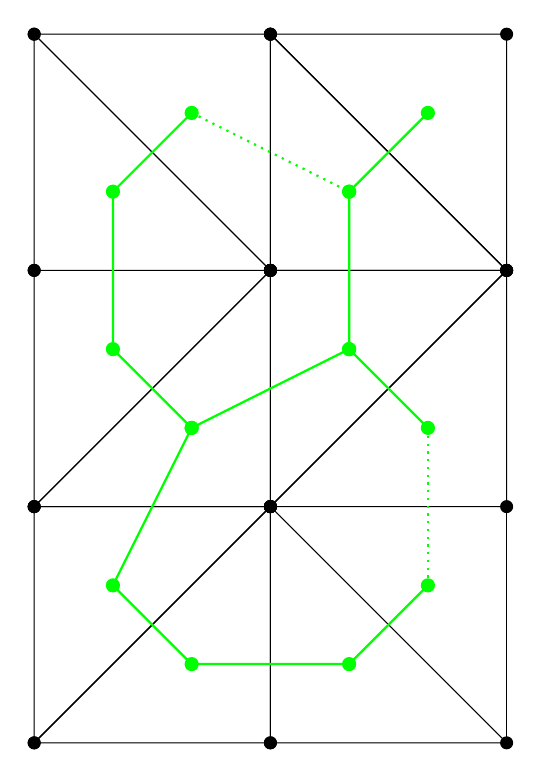
\begin{tikzpicture}
\draw[fill=black] (0,0) circle (.5ex) -- (3,0) circle (.5ex) -- (3,3) circle (.5ex) -- (0,0);
\draw[fill=black] (0,0) circle (.5ex) -- (3,3) circle (.5ex) -- (0,3) circle (.5ex) -- (0,0);

\draw[fill=black] (3,3) circle (.5ex) -- (6,3) circle(.5ex) -- (6,6) circle (.5ex) -- (3,3);
\draw[fill=black] (3,3) circle (.5ex) -- (3,6) circle(.5ex) -- (6,6)  circle (.5ex) -- (3,3);

\draw[fill=black] (3,6) circle (.5ex) -- (3,9) circle (.5ex) -- (6,6) circle (.5ex) -- (3,6);
\draw[fill=black] (6,6) circle (.5ex) -- (3,9) circle (.5ex) -- (6,9) circle (.5ex) -- (6,6);

\draw[fill=black] (3,0) circle (.5ex) -- (3,3) circle (.5ex) -- (6,0) circle (.5ex) -- (3,0);
\draw[fill=black] (6,0) -- (6,3);

\draw[fill=black] (0,6) circle (.5ex) -- (0,9) circle (.5ex) -- (3,6) circle (.5ex);
\draw[fill=black] (3,6) circle (.5ex) -- (3,9) circle (.5ex) -- (0,9) circle (.5ex);


\draw[fill=black] (0,3) circle (.5ex) -- (3,3) circle (.5ex) -- (3,6) circle (.5ex) -- (0,3);
\draw[fill=black] (0,3) circle (.5ex) -- (3,6) circle (.5ex) -- (0,6) circle (.5ex) -- (0,3);

\draw[draw=green!120, thick, fill=green] (5,4) circle (.5ex) -- (4,5) circle (.5ex) -- (4,7) circle (.5ex);

\draw[draw=green!120, thick, fill=green] (1,5) circle (.5ex) -- (2,4) circle (.5ex) -- (4,5) circle (.5ex);

\draw[draw=green!120, thick, fill=green] (2,1) circle (.5ex) -- (1,2) circle (.5ex) -- (2,4) circle (.5ex);

\draw[draw=green!120, thick, fill=green] (4,7) circle (.5ex) -- (5,8) circle (.5ex);

\draw[draw=green!120, thick, fill=green] (2,1) -- (4,1) circle (.5ex) -- (5,2) circle (.5ex);

\draw[draw=green!120, thick, fill=green] (1,5) -- (1,7) circle (.5ex) -- (2,8) circle (.5ex);

\draw[draw=green!120, thick, dotted] (2,8) -- (4,7);

\draw[draw=green!120, thick, dotted] (5,2) -- (5,4);
\end{tikzpicture}
}
\end{document}